In 1928, a letter from the Indian physicist Chandrasekhara Venkata Raman, often referred to as C.V. Raman, and his student Kariamanikkam Srinivasa Krishnan, usually mentioned as K.S. Krishnan, was published in \textit{Nature}. This letter, named \textit{A New Type Of Secondary Radiation}, outlined their findings on the topic of modified scattered radiation, which is now referred to as Raman scattering. It was the result of several years of hard work and dedication from Raman and his students, of which Krishnan is the most well known, but not the only one. Afterwards, C.V. Raman published several papers on Raman scattering and spectroscopy. For his work, C.V. Raman has recieved a Nobel Prize in Physics. \cite{ram28}
\bigskip

While this was the first time that this phenomenon has been observed, it has been predicted theoretically in 1923 by the Austrian physicist Adolf Smekal. 
\bigskip

\begin{wrapfigure}{r}{0.6\textwidth} %this figure will be at the right
    \centering
    \vspace{-25pt}
    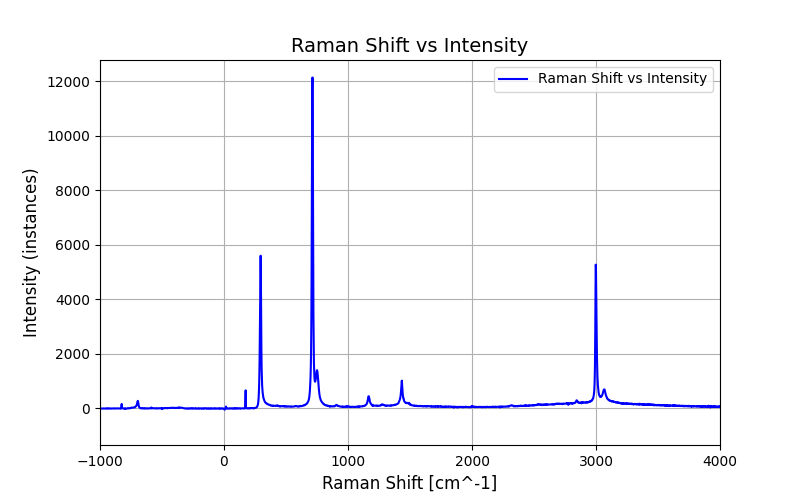
\includegraphics[width=0.55\textwidth]{images/raman_spectra/raman_shift_DCM.png}
    \caption{Example Raman spectrum (dichloromethane)}
    \label{fig:ex_dcm}
    \vspace{-15pt}
\end{wrapfigure}


Raman spectroscopy is a spectroscopic technique that observes laser light which has been scattered by an analyte. The scattered light which is being observed has different wavelengths from the incident light, and those shifts can be analyzed to obtain information about the analyte. The bonds between atoms of the molecule have certain modes of vibration which are specific to the molecule, and the energy differences between them impact the scattering. A spectrometer records a spectrum of the observed light, which is then calculated into a Raman spectrum, which shows the difference in wavenumber \( \widetilde{\nu}\) ( cm\(^{-1}\)) of the observed light and the incident laser light.



\bigskip

In the beginning, before the invention of lasers, the sun was used as a light source, with filters and lenses to focus it and to limit the wavelength, and with it the colour of the light. Using this setup and the existing spectrographs, very long integration times were needed in order to obtain measureable  spectra due to low sensitivity and the fact that Raman scattering is a very weak effect, only about 1 in 10\(^8\) photons being scattered. This made the process very inefficient. The invention of the laser in the 1960s and the general increase in sensitivity of spectrometers optimised the process and made it more competitive, compared to popular techniques like IR-Spectroscopy.
\bigskip

Now Raman spectroscopy is used in many academic fields, but also commercially.

\newpage

\subsection{Crystallography}
\textit{Crystal, any solid material in which the component atoms are arranged in a definite pattern and whose surface regularity reflects its internal symmetry.} - Britannica \cite{brittanica}

\bigskip

When a property of a crystal is checked along different axes, it does not have to yield the same results. This phenomenon is called isotrophy resp. anisotrophy, which means that the crystal does not have a defined orientation resp. that it has one. Most liquids, gases and crystalline materials with a cubic structure are isotrophic, while crystalline materials with non-cubic structures often exhibit anisotrophism. 

\bigskip

In anisotropic crystals, the molecules are fixed in specific positions. This means that their bonds can align with the polarisation of the excitation light coming from one direction, but not the other. If the bonds are aligned with the polarization of the light, their interactions are stronger than for unaligned bonds, which produces stronger Raman signals. Raman spectroscopy can be used to identify the orientations of the molecules in the material, which can give valuable information about the crystal structure in the sample and whether it has any defects. 
\cite{RSAA}

\subsection{Strain Analysis}
When stress is applied to a an object made out of a specific material, for example when it is stretched, the positions of the atoms and/or molecules in the material relative to each other are changed, which is called strain. The lenghts of the bonds between the atoms are compared to the same material without strain. This change in bond length also changes the energy differences between vibrational states, which means that they can be observed using Raman spectroscopy.

\bigskip

Strain quantification is especially important in semiconductors since it is crucial to the performance of semiconductor technology and devices which use them. 
\cite{semiconductors}

\subsection{Biochemistry and Pharmaceuticals}
 In biological systems, Raman spectroscopy can be used to detect orientations of biomolecules, their exact structures and interactions. This also includes their structural changes due to interactions with each other, heat, pressure and other influences. This can also help identify faulty molecules, and as such can help diagnose diseases.

 \bigskip

 Raman spectroscopy is also used in the pharmaceutical industry for quality control and development of new drugs. Verification of raw materials, detection of counterfeit drugs and analysis of formulations can all be done using Raman spectroscopy. it's advantage lies in the minimal sample preparation required and relatively short waiting time until the results can be accessed.\cite{pharma}

\subsection{Clinical Medicine}
As mentioned above, Raman spectroscopy can be used for the characterization and imaging of different substances found in living matter. Raman spectroscopy can be used to recognize biomarkers, which enables early diagnoses of cancers, disorders and diseases, as well as the tracking of recovery and severty rating, which would be essential to ensure better outcomes for patients. \cite{clinmed}

\bigskip

Another use of Raman spectroscopy would be in the field of regenerative medicine: research on stem cells and tissue regeneration has resulted in the emerging of new, better therapies for chronic diseases. Right now, bone marrow and organ transplantation cannot be substituted by anything else. The availability and quality of organs have to be considered though and transplantations almost always require major surgery. The goal of regenerative medicine would be to be able to grow cells and tissues in vitro, to later be transplanted, and to be able to simulate tissue regeneration. Raman spectroscopy would be a good method do investigate the biochemical functions of such tissues and cells, since most other available techniques are very invasive. As an example, one can use Raman spectroscopy to differentiate between stem cells and their derivatives. \cite{npj}

\subsection{Environmental Science}

In order to monitor pollution, for example water pollution, Raman spectroscopy can be used. It has been used to detect and identificate microplastics.\cite{micropl}

\bigskip

The advantage of Raman spectroscopy resp. its variations lies in the ease of use and smaller equipement, as well as the precision that is achievable. That makes field measurements possible, something that is impossible with other methods. Water has a very weak Raman spectrum, which makes Raman ideal for assessing situations where water acts as a solvent. Heavy metal pollution, industrial waste, pharmaceuticals and other pollutants can be detected using Surface Enhanced Raman Spectroscopy (SERS). \cite{RSAA}